%
% LaTeX report template 
%
\documentclass[a4paper,12pt]{article}
\usepackage{graphicx}
\usepackage[english]{babel}
\usepackage{fontspec}
\usepackage{listings}
\usepackage{xcolor}
%
% set python code style
\definecolor{codegreen}{rgb}{0,0.6,0}
\definecolor{codegray}{rgb}{0.5,0.5,0.5}
\definecolor{codepurple}{rgb}{0.58,0,0.82}
\definecolor{backcolour}{rgb}{0.95,0.95,0.92}

\lstdefinestyle{pystyle}{
	backgroundcolor=\color{backcolour},   
	commentstyle=\color{codegreen},
	keywordstyle=\color{magenta},
	numberstyle=\tiny\color{codegray},
	stringstyle=\color{codepurple},
	basicstyle=\ttfamily\footnotesize,
	breakatwhitespace=false,         
	breaklines=true,                 
	captionpos=b,                    
	keepspaces=true,                 
	numbers=left,                    
	numbersep=5pt,                  
	showspaces=false,                
	showstringspaces=false,
	showtabs=false,                  
	tabsize=2
}

\lstset{style=pystyle}
%
%font
\setmainfont{Times New Roman}
%
%figure space
%
\setlength{\abovecaptionskip}{0.cm}
\setlength{\belowcaptionskip}{-1cm}   %???????????
%start document
\begin{document}
%
   \title{\textbf{DSP assignment1 report}}

   \author{Jingyan Wang, 2533494w \\ Qianqian Wang , 2595993W}
          
   \date{}

   \maketitle
   
   \tableofcontents
 
  \newpage
% after a "%" symbol is treated as comment

\section{Task1}
The record can be found in 
\section{Task2}
\section{Task3}
\section{Task4}

To amplify the amplitude of the waveform,  we create a window function(Figure\ref{fig_window}) whose amplitude is 6 in 200-900Hz and 6K-10KHz. Then, we multiply it with the frequency domain of the original signal (amplify the original signal 6 times in both base and higher frequency range). Finally, we turn it back to a time series by ifft:
\begin{lstlisting}[language=Python]
w = np.ones(N)
modifyWindow(w, 200, 900, rate, 6)
modifyWindow(w, 6000, 10000, rate, 6)

lchannelfRefine = lchannelf*w
rchannelfRefine = rchannelf*w

lchannelRefine = np.fft.ifft(lchannelfRefine)
rchannelRefine = np.fft.ifft(rchannelfRefine)

def modifyWindow(w, startFreqency, endFreqency, sampleRate, value):
"""modify the window function into rectangular form"""
beginPoint = int(startFreqency//(sampleRate/N))
endPoint = int(endFreqency//(sampleRate/N))

w[beginPoint:endPoint] = value
w[-endPoint:-beginPoint] = value
\end{lstlisting}
we can find difference in both time domain and frequency domain with Figure\ref{fig_recordTR} and Figure\ref{fig_recordFR}\\
 the ouput wavefile in \lstinline{"./Output/refinedVoice.wav"}
\begin{figure}[h]   
	\centering 
	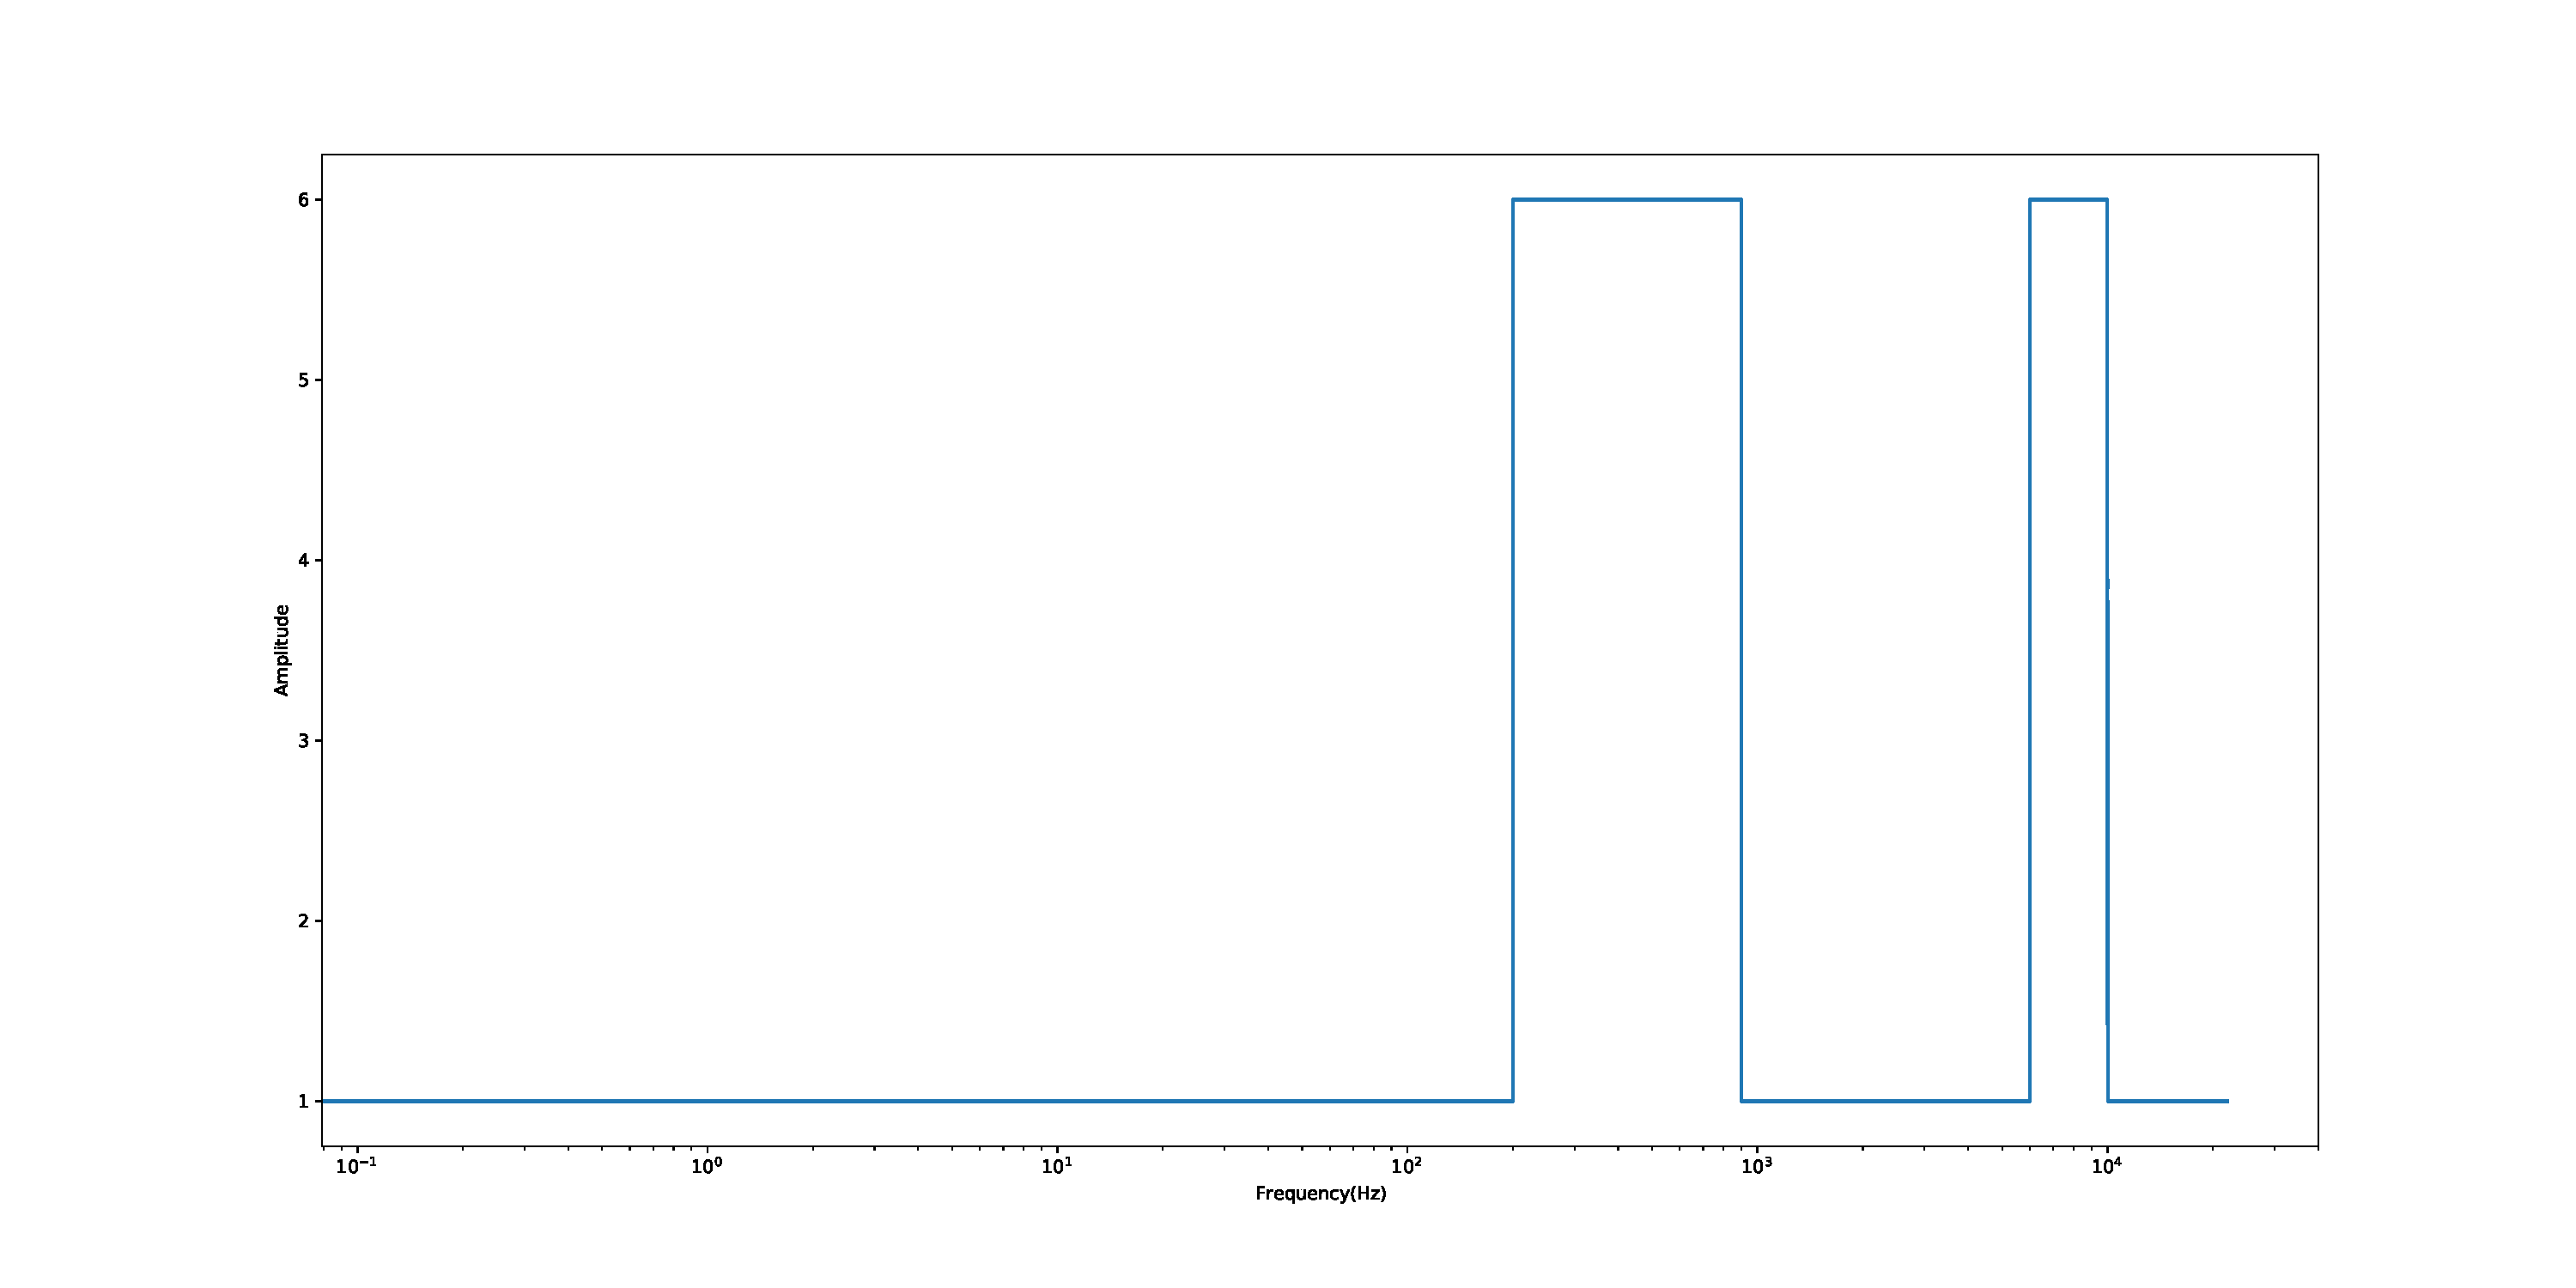
\includegraphics[width=12cm]{../Output/Figures/window.pdf} 
	\caption{window}   
	\label{fig_window}
\end{figure}

\begin{figure}[h]   
	\centering 
	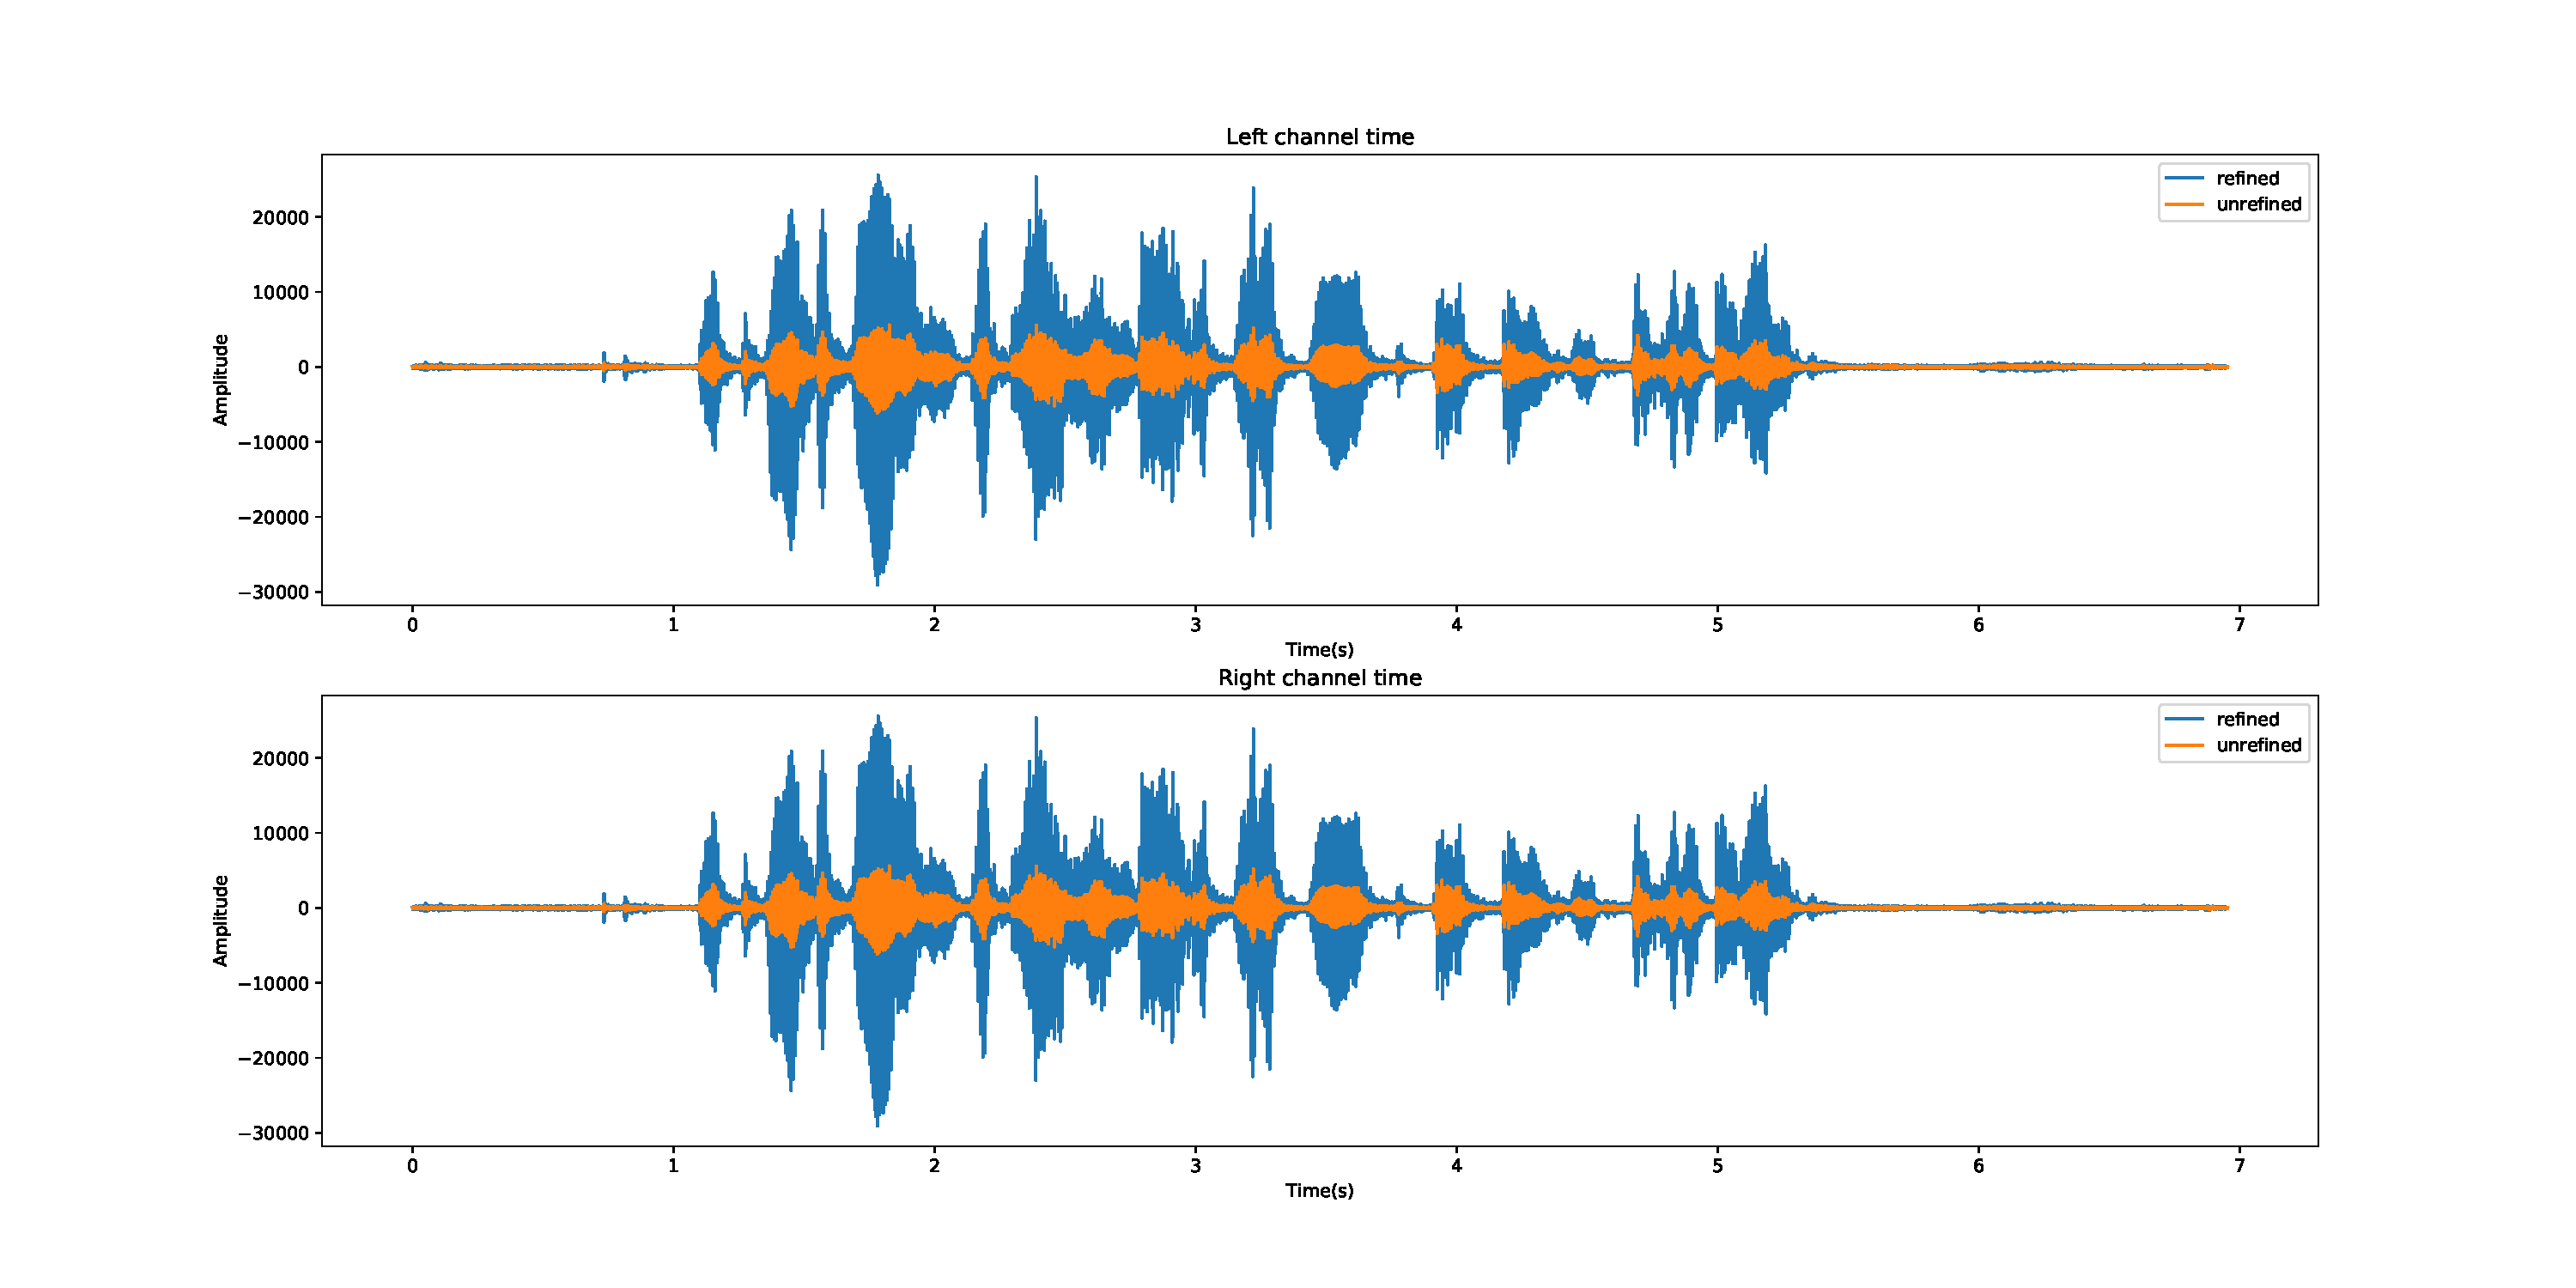
\includegraphics[width=12cm]{../Output/Figures/recordTR.pdf} 
	\caption{recordTR}   
	\label{fig_recordTR}
\end{figure}

\begin{figure}[h]   
	\centering 
	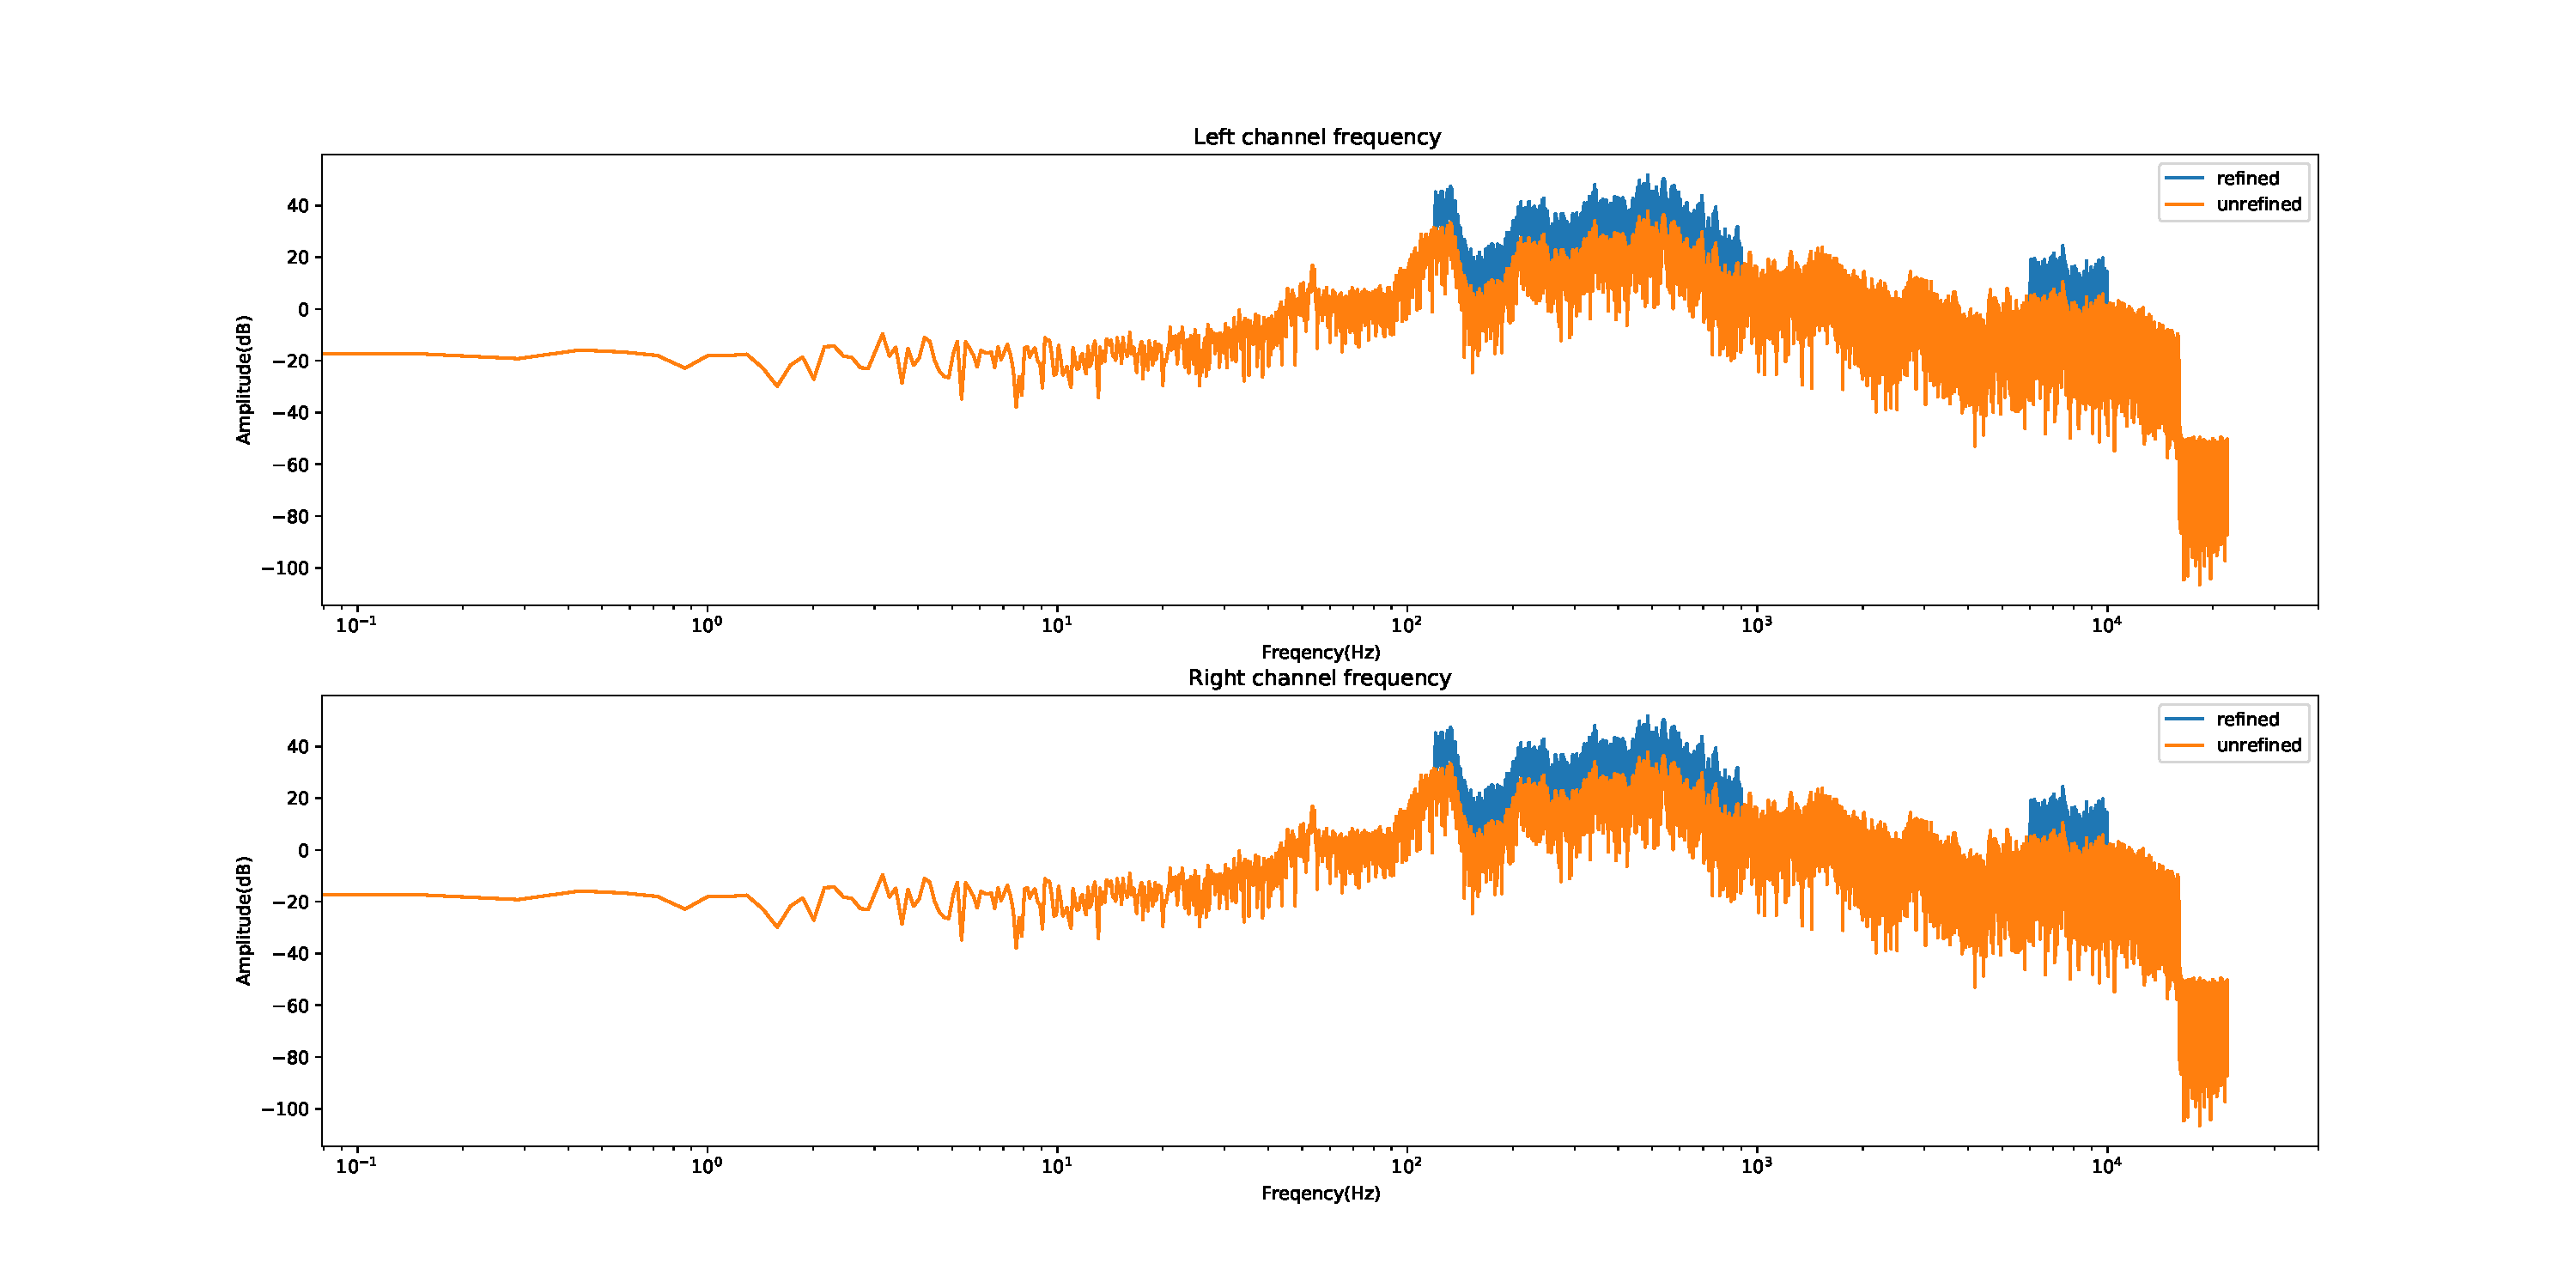
\includegraphics[width=12cm]{../Output/Figures/recordFR.pdf} 
	\caption{recordFR}   
	\label{fig_recordFR}
\end{figure}

\clearpage
\section{Code}
\lstinputlisting[language=Python]{../Assignment1.py}


\end{document}

